\documentclass[12pt,a4paper]{article}
\usepackage[utf8]{inputenc}
\usepackage[T1]{fontenc}
\usepackage[francais]{babel}
\usepackage{amsmath}
\usepackage{amsfonts}
\usepackage{amssymb}
\usepackage{graphicx}
\usepackage[top=2.00cm]{geometry}
\usepackage{titlesec}
\usepackage{calrsfs}
%%modif des titres de section diminuer la taille

\renewcommand{\thesection}{\Roman{section}}
\titleformat{\section}
{\normalfont\bfseries\Large\scshape}{\thesection}{1em}{}
\titleformat{\subsection}
{\normalfont\bfseries\large}{\thesubsection}{1em}{}

\makeatletter
\def\@maketitle{
	
	\begin{center}
		% NoLogo
		% \vspace*{+2cm}
		
		% Corner Logo
		% \begin{flushright}
		%  
\includegraphics[width=40mm]{logo_corner}\\[4ex]
		% \end{flushright}
		
		% Top Logo
		
\includegraphics[scale=0.3]{res/logo_top}
		
		
		{\LARGE \@title }\\[4ex]
		{\large \@author}\\[4ex]
		{\large \@date}\\[8ex]
		\rule{\linewidth}{0.4pt}
	\end{center}
}
\makeatletter

\author{CHARNAY Valentin, FINOT Sylvain}
\title{Compte rendu de TP :\\ \scshape Lunette Astronomique}

\date{\today}
\begin{document}
	\maketitle
	\section{Principe}
	La lunette astronomique est un système optique utilisé pour observer des objets très lointains (à l'infini). Ce système est constitué de deux lentilles convergentes:
	\begin{itemize}
		\item L'objectif, crée une image (réelle) de l'astre dans son plan focal.
		\item L'oculaire, dont le foyer objet $F_2$ coïncide avec le foyer image $F^{'}_1$
		de l'objectif.
	\end{itemize}
	Étant donné que l'image de l'objet par l'objectif est située au foyer objet de l'oculaire, l'image de l'objet par l'oculaire est virtuelle située à l'infini : la lunette astronomique est donc un système afocal.
	\section{Montage}
	\subsection{Montage}
	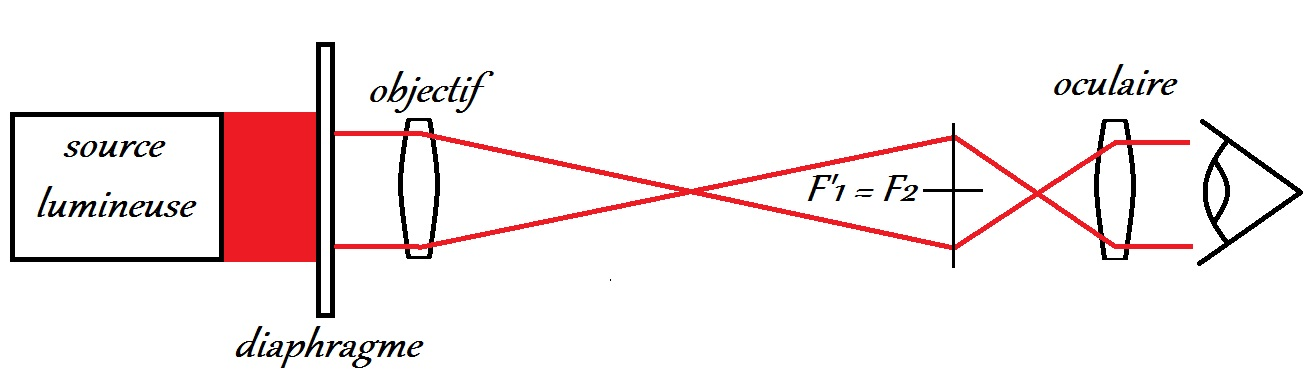
\includegraphics[scale=0.5]{schema5}
	Dans notre montage, le diaphragme sert à concentrer le signal lumineux et l'œil est remplacé par une lentille suivie d'un écran (afin de rendre plus visible pour tout le résultat et de permettre la suite du TP avec un laser).
	
	\subsection{Réglages}
	Pour trouver la bonne distance à laquelle mettre les différents objets optiques, rien de mieux que l'autocollimation. Le principe est très simple : en plaçant un miroir coté extérieur de l'objet optique, on observe l'image reçue par l'objet dans le précédent (voir schéma). Il nous faut alors bouger notre objet pour être précisément sur la focale de la lentille précédente soit avoir une image la plus nette et la plus petite possible (et si possible centré).
	
	En appliquant plusieurs fois cette méthode, on arrive à régler nos objets de telle sorte à obtenir un grossissement de notre signal lumineux de départ.
	
	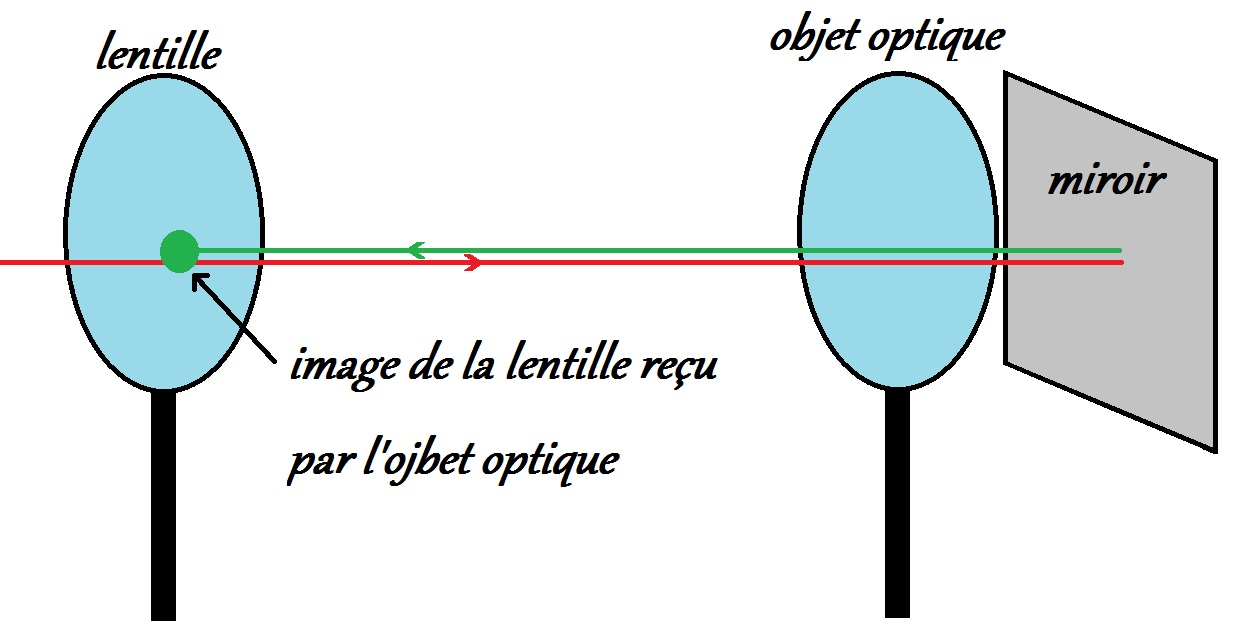
\includegraphics[scale=0.6]{schema1}
	
	\section{Montage image initiale + image grossit}
	Afin de déterminer expérimentalement le grossissement intrinsèque de notre lunette astronomique, on place après la lentille $\mathcal{L}_{0}$ une séparatrice (lame semi-réfléchissante) qui divise notre signal lumineux en deux : une partie continue tout droit dans la lunette astronomique alors que l'autre partie va taper dans un miroir, puis dans un autre afin de contourner le grossissement dû à la lunette. Le second miroir fait rentrer le signal non grossi (donc initial) dans le montage avec une autre séparatrice qui envoie les deux signaux dans la lentille "œil" $\mathcal{L}_{3}$ (voir schéma ci-dessous)\.\
	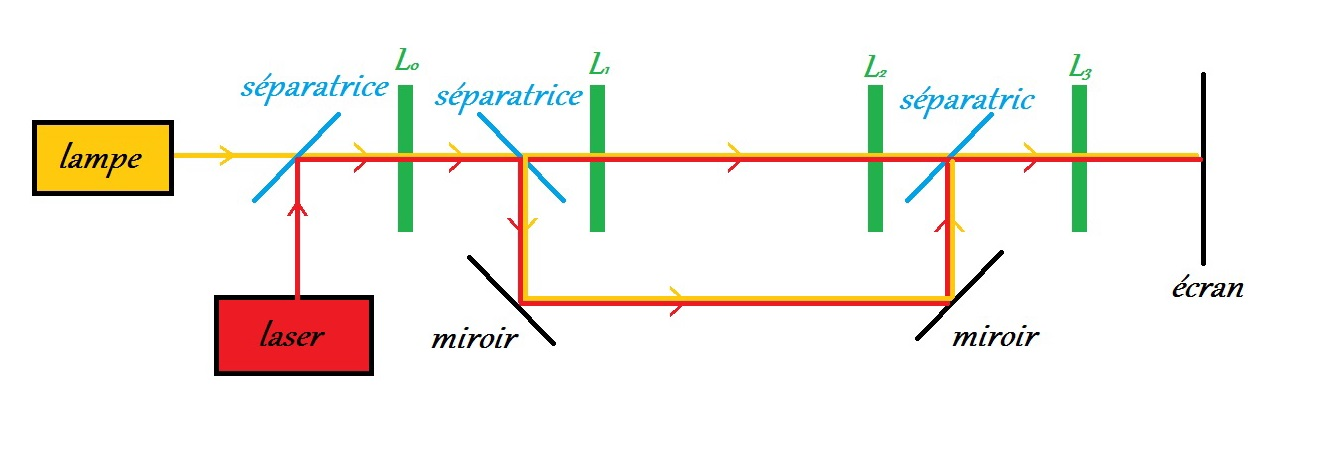
\includegraphics[scale=0.7]{schema3}\\
	On observe alors une superposition des deux images : l'une grossie et l'autre originel. 
	
	En ajoutant à notre montage un signal ponctuel (laser) à l'aide d'une séparatrice encore une fois, on peut alors visualiser le grossissement de la lunette sur un objet ponctuel (telle une étoile dans le ciel).
	
	\begin{center}
		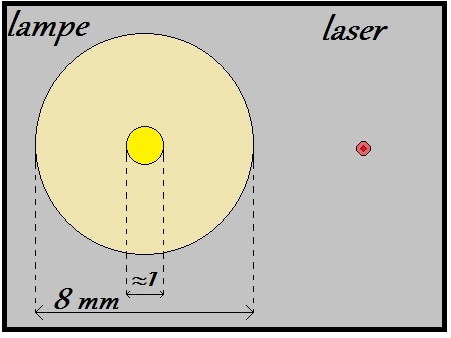
\includegraphics[scale=0.7]{schema2}
	\end{center}
	
	Dans notre expérience, les images des deux signaux (lampe et laser) sont confondues et non décalées comme sur le schéma.
	
	On remarque bien un grossissement du signal laser même si celui-ci est très peu distinguable.
	\subsection*{Calcul du grossissement intrinsèque du montage :}
	
	Bien que nous ayons défini par un grossissement d'environ 8, notre mesure de l'image initiale n'est pas précise (en-dessous du millimètre)et en étudiant théoriquement le problème on arrive à trouver un grossissement valant : 
	
	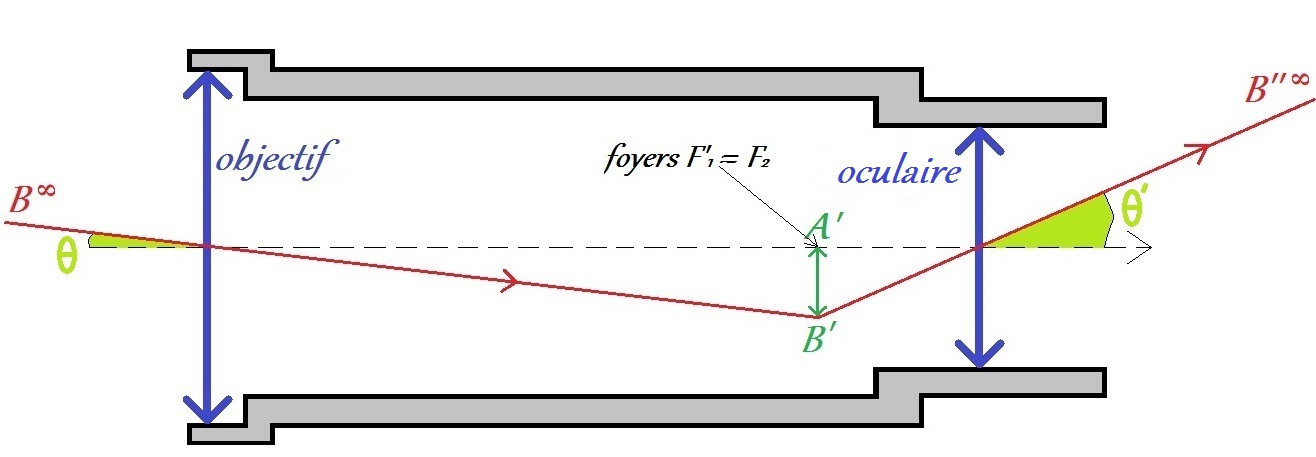
\includegraphics[scale=0.5]{schema4}
	
	D'après le schéma de la lunette ci-dessus, avec $ G \equiv \frac{\theta'}{\theta}$, on a :
	$$ \theta = arctan\left(\frac{A'B'}{f_{1}'}\right) \approx \frac{A'B'}{f_{1}'}$$
	et $$ \theta' = arctan\left(\frac{AB}{f_{2}}\right) \approx \frac{AB}{f_{2}}$$ 
	d'où $$ \boxed{ G = \frac{f_2}{f_1'}}$$
	
	En prenant un objectif de focal 100 cm et un oculaire de 10 cm on devrait, théoriquement avoir un grossissement de 10. Or, n'oublions pas qu'il s'agit d'un calcul théorique et que notre mesure n'est peu précise. Par conséquent, on notre grossissement mesuré de 8 est correct.
\end{document}

